%% SynthProof — IEEE conference (double-column) paper
%% Compile on Overleaf (recommended): New Project -> Upload -> set compiler to pdfLaTeX.
%% IEEEtran.cls ships with Overleaf and every TeX Live/MiKTeX install; no extra files needed.
%% Placeholders you MUST fill before submission are marked  %% TODO.
\documentclass[conference]{IEEEtran}
\IEEEoverridecommandlockouts

\usepackage{cite}
\usepackage{amsmath,amssymb,amsfonts}
\usepackage{algorithmic}
\usepackage{graphicx}
\usepackage{textcomp}
\usepackage{xcolor}
\usepackage{booktabs}
\usepackage{array}
\usepackage{url}
\usepackage{tikz}
\usetikzlibrary{arrows.meta,positioning,calc,fit,backgrounds,shapes.geometric,decorations.pathreplacing}
\usepackage{pgfplots}
\pgfplotsset{compat=1.17}
\usepackage[hidelinks]{hyperref}

%% -- shared TikZ styles (Brass/Ivory/Ink identity, print-safe) --
\definecolor{ink}{RGB}{26,23,18}
\definecolor{brass}{RGB}{138,90,43}
\definecolor{seal}{RGB}{124,45,42}
\definecolor{verify}{RGB}{63,107,78}
\definecolor{paper}{RGB}{244,241,234}
\tikzset{
  box/.style={draw=ink,rounded corners=2pt,fill=paper,inner sep=5pt,align=center,font=\footnotesize,minimum height=8mm},
  mech/.style={box,draw=brass,line width=0.9pt,fill=brass!8},
  leak/.style={draw=seal,rounded corners=2pt,fill=seal!8,inner sep=4pt,align=center,font=\scriptsize\itshape,text=seal},
  ok/.style={draw=verify,rounded corners=2pt,fill=verify!8,inner sep=4pt,align=center,font=\scriptsize},
  flow/.style={-{Stealth[length=2.2mm]},ink,line width=0.7pt},
  leakarrow/.style={-{Stealth[length=2mm]},seal,line width=0.7pt,dashed},
}

\def\BibTeX{{\rm B\kern-.05em{\sc i\kern-.025em b}\kern-.08em T\kern-.1667em\lower.7ex\hbox{E}\kern-.125emX}}

\newcommand{\eps}{\varepsilon}
\newcommand{\code}[1]{\texttt{\small #1}}

\begin{document}

\title{Beyond the Mechanism: Machine-Checkable\\ Release-Boundary Auditing for\\ Differentially Private Synthetic Data}

\author{
\IEEEauthorblockN{Raj Modi, Krishna Renuse, Levinesh G\,R, Aaditya Kumar Sinha, Shilpa Sonawani}
\IEEEauthorblockA{\textit{School of Computer Engineering and Technology} %% TODO: confirm dept/school
\\ \textit{MIT World Peace University}, Pune, India %% TODO: confirm institution
\\ \small Dr.~Shilpa Sonawani (Guide / Supervisor)}
\thanks{This work was carried out as a B.Tech capstone project under the guidance of
Dr.~Shilpa Sonawani. Correspondence via the department.}
}

\maketitle

\begin{abstract}
Differential privacy (DP) bounds what an adversary can learn from a mechanism's output. Yet a
synthetic-data release, in practice, is not a mechanism but a document: a table together with a
metadata card that records how it was produced. We argue that this document is itself an attack
surface, and we show why. When the metadata publishes the random seed, as machine-learning
reproducibility norms encourage, the release becomes a deterministic function of the input. An
adversary who knows every record but one can then rebuild the release for each candidate table and
read membership off an exact match. On our own pipeline the attack succeeds in all $15$ trials at
$\eps{=}1.0$ and never once for the neighbouring table. We go on to ask whether any dataset-
documentation standard in common use, from Croissant and Hugging Face cards to Datasheets, Model
Cards, and the recent DP privacy label, can even express that a release artefact is safe. None can.
Our contributions are threefold. First, we define the release boundary for DP synthetic data under
add/remove-one adjacency and enumerate the channels that cross it. Second, we build
\code{boundary-audit}, a static linter that inspects a published sheet or Croissant record without
touching the data or the producing code, and we make its one-sided nature explicit: it can prove a
channel open, but never prove one closed. Third, we ship a signed, Croissant-embeddable Privacy Data
Sheet that records the boundary properties along with the operating range of its own empirical audit.
A short case study of the field's flagship DP releases finds the same pattern everywhere: the
guarantee's parameters are documented, the artefact's safety is not. We also look one step earlier in
the pipeline, at how missing values are handled, and find, under a sanity-checked auditor, no leakage
above the DP-charged baseline, a bounded negative result for a step no prior audit has covered. None
of this is a new privacy theorem. It is integration and measurement, and we are careful about where
its limits lie.
\end{abstract}

\begin{IEEEkeywords}
differential privacy, synthetic data, membership inference, metadata standards, reproducibility,
privacy auditing, Croissant
\end{IEEEkeywords}

\section{Introduction}
Differentially private (DP) synthetic data has become a popular way to share sensitive tabular data.
A curator fits a private generative model and publishes a synthetic table that reproduces the real
one's statistics well enough to be useful, while a formal $(\eps,\delta)$ bound limits what any single
record contributes. Most research effort has gone into the mechanism itself, whether marginal-based,
GAN-based, or diffusion-based, and into the attacks that probe it, chiefly membership inference and
reconstruction~\cite{stadler2022,annamalai2024}.

A deployed release, though, is not a mechanism. It is an artefact: the synthetic table plus a card
describing how it was made. The DP guarantee is defined over the mechanism's internal
coins~\cite{dwork2014,dwork2006} and says nothing about the rest of what ships alongside the output.
We call that unguarded region the release boundary. This paper shows it is both exploitable in
practice and unaddressed by current documentation.

The core observation sets two community norms against each other. On one side, machine-learning
venues, model cards, and metadata formats all reward publishing a random seed so that results can be
reproduced. On the other, differential privacy depends on that same randomness staying secret. Fix the
seed and the mechanism becomes deterministic, so the guarantee degrades to
$\eps{=}\infty$~\cite{dwork2014,dodis2012,garfinkel2020}. Put the seed in the release metadata and the
standard DP adversary no longer needs a shadow-model attack. A single deterministic replay is enough.

Our work makes four contributions.
\begin{itemize}
\item We formalise the release boundary for DP synthetic data under add/remove-one adjacency and list
the channels that cross it: the run seed, the exact row count, an unkeyed table fingerprint, and
evaluation metrics computed on the real data. The seed channel we also measure directly.
\item We build \code{boundary-audit}, a static linter that reads a published Privacy Data Sheet or
Croissant record and flags these channels. It is deliberately one-sided, a property we call the
asymmetry principle: it can show a channel is open, but it cannot show one is closed.
\item We analyse whether existing documentation standards can express artefact safety, examine the
field's real DP releases as case studies, and release a signed, Croissant-embeddable Privacy Data
Sheet that carries the boundary properties and its audit's operating range.
\item Turning to the step before the mechanism, we audit how missing values are handled, a step no
prior privacy audit has covered, calibrate the audit with planted-leak sanity gates, and report a
bounded negative result: no leakage above the DP-charged baseline at the auditor's resolution.
\end{itemize}
We are deliberate about what counts as new here. That a public seed breaks DP is textbook. What we
contribute is the observation that a shipped, signed privacy artefact violated it in practice, that no
standard prevents this, and that a purely document-level check is feasible. The work is best read as
integration, measurement, and engineering, and Section~\ref{sec:limits} says where it stops.

\begin{figure*}[t]
\centering
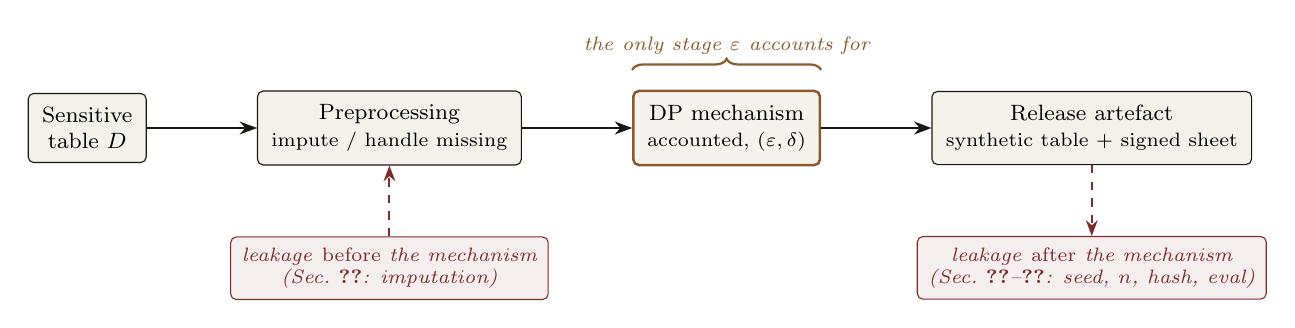
\begin{tikzpicture}[node distance=8mm and 14mm]
\node[box] (raw) {Sensitive\\table $D$};
\node[box,right=of raw] (pre) {Preprocessing\\{\scriptsize impute / handle missing}};
\node[mech,right=of pre] (dp) {DP mechanism\\{\scriptsize accounted, $(\varepsilon,\delta)$}};
\node[box,right=of dp] (rel) {Release artefact\\{\scriptsize synthetic table $+$ signed sheet}};
\draw[flow] (raw)--(pre);
\draw[flow] (pre)--(dp);
\draw[flow] (dp)--(rel);
\draw[decorate,decoration={brace,amplitude=4pt},brass,line width=0.8pt]
  ([yshift=2.5mm]dp.north west) -- ([yshift=2.5mm]dp.north east)
  node[midway,above=2pt,font=\scriptsize\itshape,text=brass]{the only stage $\varepsilon$ accounts for};
\node[leak,below=9mm of pre] (bl) {leakage \emph{before} the mechanism\\(Sec.~\ref{sec:imp}: imputation)};
\draw[leakarrow] (bl)--(pre);
\node[leak,below=9mm of rel] (al) {leakage \emph{after} the mechanism\\(Sec.~\ref{sec:boundary}--\ref{sec:cases}: seed, $n$, hash, eval)};
\draw[leakarrow] (rel)--(al);
\end{tikzpicture}
\caption{The pipeline brackets the mechanism. Differential privacy accounts only for the mechanism
(centre), yet a real deployment can leak in two unaccounted places: the preprocessing step before it
and the released artefact after it. This paper audits both.}
\label{fig:pipeline}
\end{figure*}

\section{Background and Threat Model}
\subsection{Differential privacy over internal randomness}
A randomised mechanism $\mathcal{M}:\mathcal{X}\!\to\!\mathcal{Y}$ is $(\eps,\delta)$-DP when, for
every pair of neighbouring datasets $D,D'$ and every measurable $S\subseteq\mathcal{Y}$,
\begin{equation}
\Pr_{r\sim\mathcal{R}}[\mathcal{M}(D;r)\in S] \le e^{\eps}\Pr_{r\sim\mathcal{R}}[\mathcal{M}(D';r)\in S]+\delta,
\end{equation}
with the probability taken only over the mechanism's internal coins $r$~\cite{dwork2014,dwork2006}.
Our accountant composes under add/remove-one adjacency, where two neighbours differ by a single
record. A direct consequence, and one that matters below, is that the exact row count $n$ is itself
private.

\subsection{The release artefact and the adversary}
We work in the central model. The curator holds the real table and publishes two things: the synthetic
table and a signed metadata card, the Privacy Data Sheet, which may be serialised as a Croissant
record~\cite{croissant}. Our adversary is the usual DP adversary, knowing all records but one and
trying to place the target. The difference from the mechanism-level literature is where it looks. It
attacks the released artefact and uses only what ships, with no sight of the real table or the code
that made it.

\section{The Release Boundary}\label{sec:boundary}
We say a release respects the boundary when every field of the artefact is one of three things: a
charged DP output (or a post-processing of one), a declaration the operator made before reading the
data, or a value explicitly marked in the artefact as computed on the sensitive table and not covered
by $\eps$. Anything that would let an adversary who already knows the other records test for the last
one has to sit in the first category or be withheld. In practice, four channels break this rule:

\begin{description}
\item[C1 (seed).] The run seed, from which every noise draw derives (Section~\ref{sec:seed}).
\item[C2 (exact $n$).] The exact row count, private under add/remove-one, which reaches the artefact
through the sheet, through the synthetic table's length, and through a refusal gate's row threshold.
\item[C3 (fingerprint).] An unkeyed cryptographic hash of the input table, which is a deterministic
membership test for an adversary who can hash a candidate table.
\item[C4 (evaluation).] Utility, correlation, and membership-inference metrics computed on the real
table and its holdout, released with no statement that $\eps$ does not cover them.
\end{description}

\section{The Seed-Replay Vulnerability}\label{sec:seed}
Publishing $r$ makes the conditional mechanism $\mathcal{M}_r(D)=\mathcal{M}(D;r)$ deterministic.
Whenever $\mathcal{M}(D;r)\neq\mathcal{M}(D';r)$, choosing $S=\{\mathcal{M}(D;r)\}$ gives probabilities
of $1$ and $0$, so the privacy loss is unbounded. No statistical machinery is required; the adversary
simply replays the computation.

\paragraph{Measurement} We measured the attack on our own pipeline, before the fix. For three
mechanisms (independent marginals, pairwise, and AIM) and five trials each, we build a table $D$ and
its one-record-removed neighbour $D'$, release from $D$ at a fixed public output size and a fixed seed,
then let the adversary rebuild the release from both candidates using the published seed. The counts
are stark (Table~\ref{tab:replay}): all $15$ releases reproduce exactly from the true table and none
from the neighbour, so membership is settled with certainty at a nominal $\eps{=}1.0$. Two of the
mechanisms were replayable already; the third became replayable only once we had made its sampler
deterministic for an unrelated reason, which is itself a reminder of how directly reproducibility work
cuts against DP secrecy.

\begin{table}[t]
\caption{Seed replay: exact-match count over 15 releases ($\eps{=}1.0$).}
\label{tab:replay}
\centering
\begin{tabular}{lccc}
\toprule
Rebuild with published seed & True table & Neighbour & Wrong seed \\
\midrule
Exact matches (of 15) & \textbf{15} & 0 & 0 \\
\bottomrule
\end{tabular}
\end{table}

\begin{figure}[t]
\centering
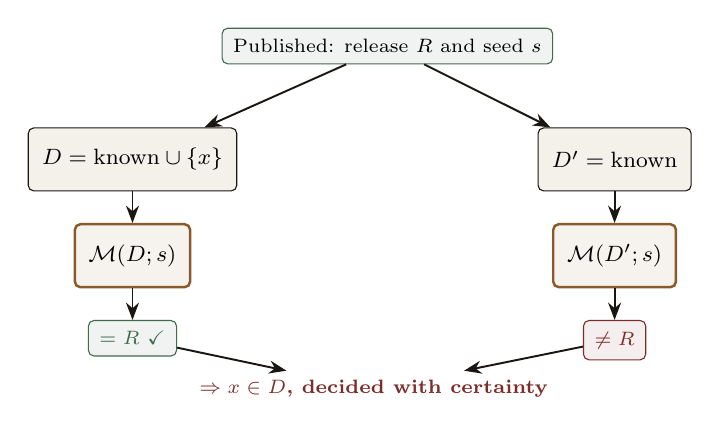
\begin{tikzpicture}[node distance=5mm and 4mm, every node/.style={font=\scriptsize}]
\node[ok] (pub) {Published: release $R$ and seed $s$};
\node[box, below left=8mm and -2mm of pub] (d) {$D=\text{known}\cup\{x\}$};
\node[box, below right=8mm and -2mm of pub] (dn) {$D'=\text{known}$};
\node[mech, below=4mm of d] (rd) {$\mathcal{M}(D;s)$};
\node[mech, below=4mm of dn] (rdn) {$\mathcal{M}(D';s)$};
\node[ok, below=4mm of rd, text=verify] (mm) {$=R$\ \checkmark};
\node[leak, below=4mm of rdn] (nm) {$\neq R$};
\draw[flow] (pub) -- (d);  \draw[flow] (pub) -- (dn);
\draw[flow] (d) -- (rd);   \draw[flow] (dn) -- (rdn);
\draw[flow] (rd) -- (mm);  \draw[flow] (rdn) -- (nm);
\node[below=4mm of $(mm)!0.5!(nm)$, font=\scriptsize\bfseries, text=seal, align=center] (c)
  {$\Rightarrow x\in D$, decided with certainty};
\draw[flow] (mm) -- (c);   \draw[flow] (nm) -- (c);
\end{tikzpicture}
\caption{Seed replay. Holding the published seed $s$, the adversary rebuilds the release for both
candidate tables; exactly one reproduces $R$, deciding membership with no statistical uncertainty.}
\label{fig:replay}
\end{figure}

\paragraph{Fix} The fix is to withhold the seed from every artefact and draw it from the operating
system when the operator supplies none. A seed the operator does provide is kept for their own
reproducibility and never written into the release. Because sampling only post-processes the private
model, keeping the seed secret costs nothing from the budget.

\section{Standards Gap Analysis}
We next asked a narrow, checkable question: can any documentation standard in common use express the
boundary properties at all? We fixed eleven properties, namely the guarantee parameters (P1~$\eps$,
P2~$\delta$, P3~mechanism), the neighbour relation (P4), and seven artefact-safety properties
(P5~release-size provenance, P6~seed secrecy, P7~keyed fingerprint, P8~evaluation-privacy label,
P9~audit operating range, P10~tamper-evidence, P11~machine-checkable enforcement), and checked each
against the actual specification of five standards. Table~\ref{tab:gap} collects the result. Every
standard can describe a dataset, and the recent expert-elicited DP label~\cite{dibia2026} is genuinely
rich on parameters, but none reaches the artefact-safety properties P5 through P11, and none is at once
tamper-evident and privacy-aware machine-checkable.

\begin{table}[t]
\caption{Can the standard express the property? Y/\,$\sim$\,/N.}
\label{tab:gap}
\centering
\setlength{\tabcolsep}{4pt}
\begin{tabular}{lccccc|c}
\toprule
 & Crois. & HF & Data- & Model & DP & \textbf{Ours} \\
Property & 1.1 & card & sheet & Card & label & \textbf{PDS} \\
\midrule
P1 $\eps$            & N & N & N & N & Y & \textbf{Y} \\
P2 $\delta$          & N & N & N & N & Y & \textbf{Y} \\
P3 mechanism         & N & N & N & $\sim$ & Y & \textbf{Y} \\
P4 neighbour rel.    & N & N & N & N & $\sim$ & \textbf{Y} \\
P5 size provenance   & N & N & N & N & N & \textbf{Y} \\
P6 seed secrecy      & N & N & N & N & N & \textbf{Y} \\
P7 keyed fingerprint & N & N & N & N & N & \textbf{Y} \\
P8 eval-privacy      & N & N & N & $\sim$ & $\sim$ & \textbf{Y} \\
P9 audit range/LoD   & N & N & N & N & N & \textbf{Y} \\
P10 tamper-evidence  & N & N & N & N & N & \textbf{Y} \\
P11 machine-check    & $\sim$ & $\sim$ & N & N & N & \textbf{Y} \\
\bottomrule
\end{tabular}
\end{table}

\section{\code{boundary-audit}: A Static, Data-Blind Linter}
\code{boundary-audit} takes a published Privacy Data Sheet or Croissant record, reads nothing else, and
reports each field that discloses something $\eps$ does not cover. It never opens the data or the
producing code. Findings come in three grades: \emph{leak}, where the artefact itself exposes a
channel; \emph{unverifiable}, where the artefact is consistent with a sound release but only the
producer's honesty makes it so; and \emph{note}, where a sound basis is stated and nothing in the
artefact contradicts it.

\paragraph{The asymmetry principle} The check is one-sided by nature. It can establish that a channel
is open, since a published seed is plainly a published seed. It cannot establish that a channel is
closed: a keyed HMAC and an unkeyed SHA-256 are both sixty-four hex characters, and a declared row
count that happens to equal $n$ still leaks it. So the tool never pronounces a release private. It
flags the open channels and marks the rest as resting on the producer's word. We regard that restraint
as a feature rather than a shortcoming, because a checker claiming to certify privacy from a document
alone would commit exactly the overclaim the field keeps warning against.

\section{Case Study: Real DP Releases}\label{sec:cases}
The obvious move, auditing DP releases at scale on a public hub, does not work: across $286$ unique
synthetic or privacy-tagged datasets we surveyed, not one declared DP with an $\eps$ value. We
therefore examined the documentation of the field's flagship real releases instead
(Table~\ref{tab:cases}), and the pattern holds across all of them. Each documents the guarantee's
parameters, usually $\eps$ and the mechanism, but not the artefact's safety. The nearest thing to an
exception is instructive: the US Census 2020 Disclosure Avoidance System does name its invariants as
quantities released outside the budget~\cite{abowd2022}, but it does so in prose, as policy, not as a
property a tool could check. NIST's SDNist, the closest existing practice, records $\eps$, $\delta$,
and method in a label yet has no artefact-safety field either.

\begin{table}[t]
\caption{Real DP releases: parameters documented vs.\ artefact safety.}
\label{tab:cases}
\centering
\begin{tabular}{lcc}
\toprule
Release & Params ($\eps$/mech) & Artefact safety (P5--P11) \\
\midrule
US Census 2020 DAS & Yes & No (invariants in prose) \\
NIST SDNist label  & Yes & No \\
OpenDP / SmartNoise & Yes (in code) & No \\
Apple (local model) & Yes & n/a (no central table) \\
\bottomrule
\end{tabular}
\end{table}

\section{Auditing Before the Mechanism: Missing-Data Handling}\label{sec:imp}
So far the boundary has concerned what leaks after the mechanism. The pipeline also has an unaccounted
step before it: preprocessing. Recent results show that individual preprocessing steps can break
end-to-end DP, whether the step is domain extraction~\cite{ganev_domain}, discretization
\cite{ganev_discrete}, or SMOTE oversampling~\cite{ganev_smote}, because one record can decide a domain
boundary or a synthesised minority point. Missing-data handling is a fourth step that every pipeline
performs, and it has escaped this scrutiny. The single study of DP generation with missing data treats
missingness as a source of privacy amplification rather than leakage~\cite{mohapatra2024}, and no
membership-inference audit of the handling step has appeared. We supply one.

\paragraph{Design} We compare five ways of handling missingness ahead of an unchanged DP synthesiser.
A0 drops incomplete rows, a per-row stability-$1$ filter that costs utility but is not a DP violation.
A1 fills missing entries with a public sentinel category. The remaining arms impute across records,
each in an uncharged and a DP-charged form: a marginal version using the mode or median (A2 against A3)
and a model-based $k$-nearest-neighbours version (A4 against A4$_{\text{DP}}$), the latter pooling
individual neighbours and so, in principle, able to memorise them. On UCI Adult, with native
missingness and with injected MCAR, MAR, and MNAR patterns at $10$ to $20\%$, we fit each arm on
$n{=}1500$ members and test membership against $1500$ disjoint non-members over at least eight seeds,
reporting $95\%$ bootstrap intervals. Adult's native missingness is categorical, so we use a
categorical-aware membership auditor and, crucially, validate it with two planted-leak sanity gates
before trusting any null.

\paragraph{The instrument can see a leak} The auditor is not blind. A planted verbatim numeric leak is
caught at AUC $0.615\,[0.609,0.620]$ and a planted verbatim categorical leak at $0.606\,[0.596,0.618]$,
both clearly separated from a private-release null of $0.497\,[0.488,0.506]$. A leak of verbatim-copy
strength is therefore visible, which is what makes a null below it worth reporting.

\paragraph{Result} No imputation arm produces meaningful leakage, and no uncharged arm exceeds its
DP-charged counterpart. Across both mechanisms, both values of $\eps$, and every missingness pattern,
the arms sit at AUC around $0.51$ with overlapping intervals (Table~\ref{tab:imp}). Even the $k$-NN
imputer, the arm most able to memorise, stays level with its charged baseline. The likely reason is
$O(1/n)$ damping: mode, median, and neighbour-pooled imputation all inject low-entropy values whose
per-record influence is small next to the downstream DP noise, where $\sigma=O(1/\eps)$ dominates
$1/n$.

\begin{table}[t]
\caption{Missing-data audit: categorical-aware MIA AUC (member vs.\ non-member), UCI Adult, native
missingness, $\eps{=}1$, $8$ seeds. All arms overlap; none reaches the verbatim-leak level.}
\label{tab:imp}
\centering
\begin{tabular}{lcc}
\toprule
Arm & Independent & DP-VAE \\
\midrule
\emph{Sanity: verbatim leak} & \multicolumn{2}{c}{$0.606\,[0.596,0.618]$} \\
\emph{Sanity: private null}  & \multicolumn{2}{c}{$0.497\,[0.488,0.506]$} \\
\midrule
A2 marginal, uncharged        & 0.510 & 0.508 \\
A3 marginal, DP-charged       & 0.509 & 0.507 \\
A4 $k$-NN, uncharged          & 0.509 & 0.507 \\
A4 $k$-NN, DP-charged         & 0.508 & 0.506 \\
\bottomrule
\end{tabular}
\end{table}

\begin{figure}[t]
\centering
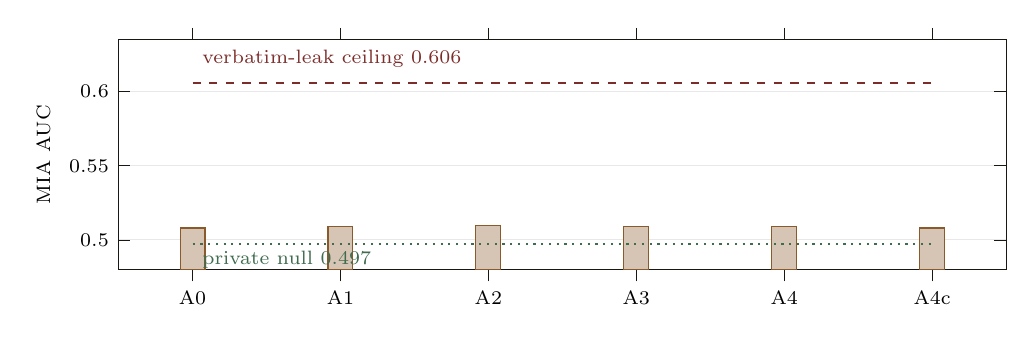
\begin{tikzpicture}
\begin{axis}[
  width=1.06\columnwidth, height=4.5cm,
  ybar, bar width=9pt,
  ymin=0.48, ymax=0.635,
  ylabel={\scriptsize MIA AUC},
  symbolic x coords={A0,A1,A2,A3,A4,A4c},
  xtick=data, x tick label style={font=\scriptsize},
  ytick={0.50,0.55,0.60}, y tick label style={font=\scriptsize},
  ymajorgrids, grid style={gray!18},
  enlarge x limits=0.10, axis line style={ink}, tick style={ink},
]
\addplot[fill=brass!35,draw=brass] coordinates
  {(A0,0.508)(A1,0.509)(A2,0.510)(A3,0.509)(A4,0.509)(A4c,0.508)};
\draw[seal,thick,dashed] (axis cs:A0,0.606) -- (axis cs:A4c,0.606);
\node[seal,font=\scriptsize,anchor=west] at (axis cs:A0,0.622) {verbatim-leak ceiling 0.606};
\draw[verify,thick,dotted] (axis cs:A0,0.497) -- (axis cs:A4c,0.497);
\node[verify,font=\scriptsize,anchor=west] at (axis cs:A0,0.487) {private null 0.497};
\end{axis}
\end{tikzpicture}
\caption{Missing-data audit (Independent, $\eps{=}1$, native). Every handling arm (A4c $=$ A4
DP-charged) sits at the private-null floor, far below the level at which the sanity-gated auditor
resolves a verbatim leak. Uncharged arms do not exceed their charged counterparts.}
\label{fig:imp}
\end{figure}

\paragraph{Honest scope} This is a bounded negative result, not a proof of safety. The auditor
resolves leaks near a verbatim copy, so anything subtler, between roughly $0.51$ and $0.60$ in AUC,
could slip past it, and the study covers one dataset at a single $n$ and two values of $\eps$. Stated
carefully: missing-data handling, which no prior audit had examined, shows no membership leakage above
the DP-charged baseline at this auditor's resolution, in contrast to domain extraction and SMOTE, which
do leak. The complete-case drop arm A0 loses utility but is not a DP violation, and we do not present
it as one.

\section{The Signed Privacy Data Sheet}
The Privacy Data Sheet is a machine-readable record that carries all eleven properties, is signed with
an Ed25519 key so that altering any field is detectable, and serialises as a Croissant~1.1 extension
that ordinary Croissant tooling can already read. Two choices are worth calling out. The input
fingerprint is a keyed HMAC under a curator secret, which lets the curator still recognise a repeat
release of the same table while giving a third party nothing to test membership with. And the sheet
reports not just an audited $\eps$ but the operating range of the audit behind it, because an empirical
privacy figure with no stated resolution can pass for safety, a failure the expert study
of~\cite{dibia2026} calls ``privacy theater.'' We borrow the limit-of-detection convention from
analytical measurement~\cite{miqe2025}, so that an audited $\eps=0.0$ sitting beside a ceiling of
$2.97$ at $60$ canaries reads as below the instrument's resolution rather than as an absence of
leakage.

\section{Related Work}
Mechanism-level DP auditing estimates an algorithm's empirical privacy by attacking its outputs or by
grey-box inspection of its code~\cite{annamalai2024,cebere2026}, and membership inference against
synthetic data is by now a well-developed area~\cite{stadler2022}. All of it runs code on private
data; we instead read a published document with no such access. The documentation standards,
Croissant~\cite{croissant}, Datasheets~\cite{gebru2021}, and Model Cards~\cite{mitchell2019}, describe
datasets but carry no DP fields, while the expert-elicited DP label~\cite{dibia2026} communicates
parameters to a human reader yet is neither signed nor machine-checkable and, on its authors' own
account, lacks an operating-range convention. Statistical disclosure control gates analytical outputs
rather than metadata artefacts. The pull between reproducibility and randomness secrecy is documented
at the level of the mechanism~\cite{garfinkel2020,mironov2012}; our contribution is to show it
surfacing in a shipped artefact and to give a check for it.

\section{Positioning and Novelty}\label{sec:novelty}
We try to be exact about what is and is not new (Table~\ref{tab:novelty}). We claim no new privacy
theorem, since a published seed collapsing DP falls straight out of the definition. What we do claim is
four things. N1 is a systematisation: the release boundary treated as an object of study, with its
channels enumerated under a stated adjacency. N2 is an artefact-level, document-only audit tool, where
every prior DP audit we know of works on the mechanism or its code and needs the data or the gradients.
N3 is an empirical demonstration that a shipped, signed privacy artefact actually violated seed
secrecy, backed by a measured attack (Fig.~\ref{fig:replay}). N4 is a membership-inference audit of
missing-data handling, which extends the preprocessing-audit
line~\cite{ganev_domain,ganev_discrete,ganev_smote} to a step it had not reached, with a bounded
negative result. The novelty is one of combination. Prior work sits in single cells of
Table~\ref{tab:novelty}; auditing a released artefact from the artefact alone, machine-checkably and
with tamper-evidence, is the cell that stays empty. We have found no prior static, document-only linter
for DP release artefacts and no prior membership audit of missing-data handling, though we cannot rule
such work out exhaustively and mark the claim as best-effort.

\begin{table}[t]
\caption{Positioning against adjacent work. ``Blind'' $=$ auditable from the published artefact
alone (no data/code); ``M/C'' $=$ machine-checkable; ``Sig.'' $=$ signed/tamper-evident.}
\label{tab:novelty}
\centering
\setlength{\tabcolsep}{3.5pt}
\begin{tabular}{lcccc}
\toprule
Line of work & Audit target & Blind & M/C & Sig. \\
\midrule
Mechanism auditing~\cite{annamalai2024,cebere2026} & mechanism & N & $\sim$ & N \\
MIA on synthetic~\cite{stadler2022}                & output     & N & N & N \\
Metadata standards~\cite{croissant,gebru2021}      & dataset    & Y & syntax & N \\
DP privacy label~\cite{dibia2026}                  & parameters & Y & N & N \\
Preproc. audits~\cite{ganev_domain,ganev_smote}    & preprocessing & N & N & N \\
\textbf{This work} & \textbf{artefact\,$+$\,pre} & \textbf{Y} & \textbf{Y} & \textbf{Y} \\
\bottomrule
\end{tabular}
\end{table}

\section{Limitations}\label{sec:limits}
The seed-collapse argument is immediate from the definition of DP and we do not present it as new; the
finding is that it showed up in a signed release artefact and that no standard heads it off. The linter
is asymmetric by design and certifies nothing on its own. The case study is a qualitative reading of
five heterogeneous releases rather than a population estimate, and a larger study should draw from DP
deployment registries, since the open ML hubs carry almost no DP releases. Cryptographic signing is a
solved primitive and we claim only its application. Taken together the work is integration,
measurement, and engineering, and while we have found no prior static, document-only release-boundary
linter for DP artefacts, we cannot prove that absence.

\section{Conclusion}
Differential privacy secures the mechanism, but what a deployment ships is a document. We have shown
that this document can leak outside $\eps$, most sharply when a seed published for reproducibility turns
the release into a deterministic membership oracle; that no dataset-documentation standard can express
whether a release artefact is safe; and that a static, document-only linter can check for the leaks
that do occur. Alongside it we release a signed, Croissant-embeddable Privacy Data Sheet carrying the
boundary properties and the operating range of its own audit. The parameters of the guarantee are
steadily better documented. The safety of the artefact is not, and closing that gap is the aim of this
work.

\section*{Reproducibility}
The pipeline, the linter, the seed-replay probe, the standards analysis, and the case study are
available in the project repository. %% TODO: add DOI / URL when public.

\begin{thebibliography}{00}
\bibitem{dwork2014} C.~Dwork and A.~Roth, ``The algorithmic foundations of differential privacy,''
\emph{Found. Trends Theor. Comput. Sci.}, vol.~9, no.~3--4, pp.~211--407, 2014.
\bibitem{dwork2006} C.~Dwork, F.~McSherry, K.~Nissim, and A.~Smith, ``Calibrating noise to
sensitivity in private data analysis,'' in \emph{Theory of Cryptography (TCC)}, 2006, pp.~265--284.
\bibitem{dodis2012} Y.~Dodis, A.~L\'opez-Alt, I.~Mironov, and S.~Vadhan, ``Differential privacy with
imperfect randomness,'' in \emph{Advances in Cryptology (CRYPTO)}, LNCS 7417, 2012, pp.~497--516.
\bibitem{garfinkel2020} S.~L.~Garfinkel and P.~Leclerc, ``Randomness concerns when deploying
differential privacy,'' in \emph{Proc. Workshop on Privacy in the Electronic Society (WPES)}, 2020,
pp.~73--86.
\bibitem{mironov2012} I.~Mironov, ``On significance of the least significant bits for differential
privacy,'' in \emph{Proc. ACM CCS}, 2012, pp.~650--661.
\bibitem{dibia2026} O.~Dibia, M.~Lu, P.~Bhattacharjee, J.~P.~Near, and Y.~Feng, ``\,`We need a
standard': toward an expert-informed privacy label for differential privacy,'' \emph{Proc. Priv.
Enhancing Technol. (PoPETs)}, 2026. arXiv:2507.15997.
\bibitem{croissant} M.~Akhtar \emph{et al.}, ``Croissant: a metadata format for ML-ready datasets,''
MLCommons, 2024.
\bibitem{gebru2021} T.~Gebru \emph{et al.}, ``Datasheets for datasets,'' \emph{Commun. ACM}, vol.~64,
no.~12, pp.~86--92, 2021.
\bibitem{mitchell2019} M.~Mitchell \emph{et al.}, ``Model cards for model reporting,'' in \emph{Proc.
ACM FAT\textasteriskcentered}, 2019, pp.~220--229.
\bibitem{stadler2022} T.~Stadler, B.~Oprisanu, and C.~Troncoso, ``Synthetic data: anonymisation
groundhog day,'' in \emph{Proc. USENIX Security}, 2022, pp.~1451--1468.
\bibitem{annamalai2024} M.~S.~M.~S.~Annamalai, G.~Ganev, and E.~De~Cristofaro, ``What you want is not
what you get: towards tight and practical DP auditing,'' \emph{USENIX Security}, 2024. arXiv:2405.10994.
\bibitem{cebere2026} B.~Cebere \emph{et al.}, ``Privacy in theory, bugs in practice: grey-box auditing
of differential privacy libraries,'' \emph{PoPETs}, 2026. arXiv:2602.17454.
\bibitem{abowd2022} J.~M.~Abowd \emph{et al.}, ``The 2020 census disclosure avoidance system TopDown
algorithm,'' \emph{Harvard Data Science Review}, 2022. arXiv:2204.08986.
\bibitem{miqe2025} S.~A.~Bustin \emph{et al.}, ``MIQE 2.0: revision of the minimum information for
publication of quantitative real-time PCR experiments,'' \emph{Clinical Chemistry}, vol.~71, no.~6,
pp.~634--651, 2025.
\bibitem{ganev_domain} G.~Ganev, M.~S.~M.~S.~Annamalai, S.~Mahiou, and E.~De~Cristofaro,
``Understanding the impact of data domain extraction on synthetic data privacy,'' 2025.
arXiv:2504.08254.
\bibitem{ganev_discrete} G.~Ganev \emph{et al.}, ``The importance of being discrete: privacy of
discretization in differentially private synthetic data,'' in \emph{Proc. ACM CCS}, 2025.
arXiv:2504.06923.
\bibitem{ganev_smote} G.~Ganev \emph{et al.}, ``SMOTE and mirrors: exposing privacy leakage from
synthetic minority oversampling,'' 2025. arXiv:2510.15083.
\bibitem{mohapatra2024} S.~Mohapatra, J.~Zong, F.~Kerschbaum, and X.~He, ``Differentially private
data generation with missing data,'' \emph{Proc. VLDB Endow.}, vol.~17, no.~8, pp.~2022--2035, 2024.
arXiv:2310.11548.
\end{thebibliography}

\end{document}
